% mainfile: ../../../../master.tex
\subsection{RNA integrity assessment by electrophoresis}
% The part of the label after the colon must match the file name. Otherwise,
% conditional compilation based on task labels does NOT work.
\label{task:20180317_cj0}
\tags{lab,rna}
\authors{cj}
%\files{}
%\persons{}

\comment{It's saturday, so I arrive rather late around 10:00 AM, and I start right away by casting the gels and defrosting my RNA samples as well as the SYBR\cR Gold.}

\subsubsection{Introduction}

Because I failed to see the RNA on the gel yesterday, I must repeat the experiment but this time, I will use a lot more RNA than previously.

\subsubsection{1\% Agarose gel preparation}

\begin{enumerate}
\item Measure with erlenmeyer 50~mL of 1\% agarose gel.\sidenote{The 1\% agarose gel is kept at 60\degree C in the gel room.}
\item Warm up the erlenmeyer for 15s in microwave: agarose will be more fluid and it will avoid bubbles when casting the gel
\item Cast the gel with the comb (for 15 wells)
\item Let the gel set for 20 min
\end{enumerate}

\subsubsection{Sample preparation}

In a \gls{pcr} 8-well rack mix:
\begin{itemize}
\item sample of nucleic acid sample according to volumes shown in table \ref{tab:20180317_prep_samples}
\item blue dye (bromothymol blue) according to volumes shown in table \ref{tab:2018031_prep_samples}
\comment{For each sample, the final quantity of nucleic acids is 20~ng.}
\item Tap gently tubes to mix up everything
\item Centrifuge briefly to bring all the liquid to the bottom
\end{itemize}

\begin{table}[htbp]
\caption{nucleicacidssamples.csv}
\label{tab:2018031_prep_samples}
\centering
\resizebox{\textwidth}{!}{
\begin{tabular}{l l l l l l l l r r r }
\toprule
User & Label & Label colour & Box pos. & Extr. method & Start mat. & Qubit\texttrademark~ (ug/mL) & vol. a prelever & vol. loading buffer \\ 
\midrule
\texttt{CJ} & DNA MP & GREEN & C4 & MasterPure & Micro-algae culture & 3,11 & 32,15 & -17,15
 \\
\texttt{CJ} & RNA MP & GREEN & C5 & MasterPure & Micro-algae culture & 7,20 & 13,89 & 1,11
 \\
\texttt{CJ} & DNA 1802 & PURPLE & C6 & AllPrep & Micro-algae culture & 2,44 & 40,98 & -25,98
 \\
\texttt{CJ} & RNA AP & PINK & C7 & AllPrep & Micro-algae culture & 8,77 & 11,40 & 3,60
 \\
\texttt{CJ} & DNA AP & BLUE & E1 & AllPrep & Micro-algae culture & 5,86 & 17,06 & -2,06
 \\
\texttt{CJ} & RNA AP & BLUE & E2 & AllPrep & Micro-algae culture & 31,50 & 3,17 & 11,83
 \\
\texttt{CJ} & DNA MP & YELLOW & E3 & MasterPure & Micro-algae culture & 18,20 & 5,49 & 9,51
 \\
\texttt{CJ} & RNA MP & YELLOW & E4 & MasterPure & Micro-algae culture & 32,20 & 3,11 & 11,89
 \\
\texttt{CJ} & DNA & NONE & E5 & AllPrep & Micro-algae culture & 7,71 & 12,97 & 2,03
 \\
\texttt{CJ} & RNA & NONE & E6 & AllPrep & Micro-algae culture & 3,94 & 25,38 & -10,38
 \\
\texttt{CJ} & DNA & NONE & E7 & AllPrep & Micro-algae culture & 3,45 & 28,99 & -13,99
 \\
\texttt{CJ} & RNA & NONE & E8 & AllPrep & Micro-algae culture & 14,00 & 7,14 & 7,86
 \\
\texttt{CJ} & MP DNA & PEACH & F1 & MasterPure & Micro-algae culture & 17,00 & 5,88 & 9,12
 \\
\texttt{CJ} & MP RNA & PEACH & F2 & MasterPure & Micro-algae culture & 7,19 & 13,91 & 1,09
 \\
\bottomrule
\end{tabular}
}
\\
\end{table}


\subsubsection{Electrophoresis}

For this electrophoresis migration, we run:
\begin{itemize}
\item 10~\textmu L of each sample 
\item 5~\textmu L of the 1~kb ladder
\item 5~\textmu L of the 2-log ladder
\end{itemize}
\comment{I leave empty lanes between ladders and samples.}

\begin{enumerate}
\item Place the agarose gel into the gel box (electrophoresis unit) containing TAE buffer
\item Load 5~\textmu L of molecular weight ladder into the first and last lane of the gel
\item Load 9~\textmu L of each sample into the additional wells of the gel
\item Run for 60 min with the \gls{eps} 301 at 80~V, 400~mA
\item Remove gel from the migration tank and place in the staining container (a recycled tip box).
\end{enumerate}

\begin{enumerate}
\item Ensure SYBR\cR gold is properly thawed.
\item Ensure the pH of TAE buffer is between 7.5 and 8
\item Prepare the staining solution at 1X SYBR\cR Gold in TAE buffer.
\comment{I actually use the staining solution solution I made yesterday and kept in aluminium foild at room tempature.}
\item Transfer 100 mL of staining solution in the staining container.
\item Incubate under agitation for 10 to 40 min.
\comment{Gel with DNA was incubated 20 min but since it was hard to take a good picture, I decided to incubate the gel another 20 min to see the difference and it did not change much. Therefore for the gel with RNA, the incubation lasted 30 min.}
\item Visualize your nucleic acid fragments with \gls{uv} lights.
\end{enumerate}
\comment{The CCD camera by BioRad does not work anymore. In the meanwhile, we use transilluminator and take the picture with my cell phone.}

\subsubsection{Results}

\begin{figure}[H] % position of the figure 
    \centering
    \caption{1\% agarose gel with RNA after 30 min. incubation in the 1X SYBR\cR Gold.}
    \label{fig:20180317_gel_sybr_gold_rna}
    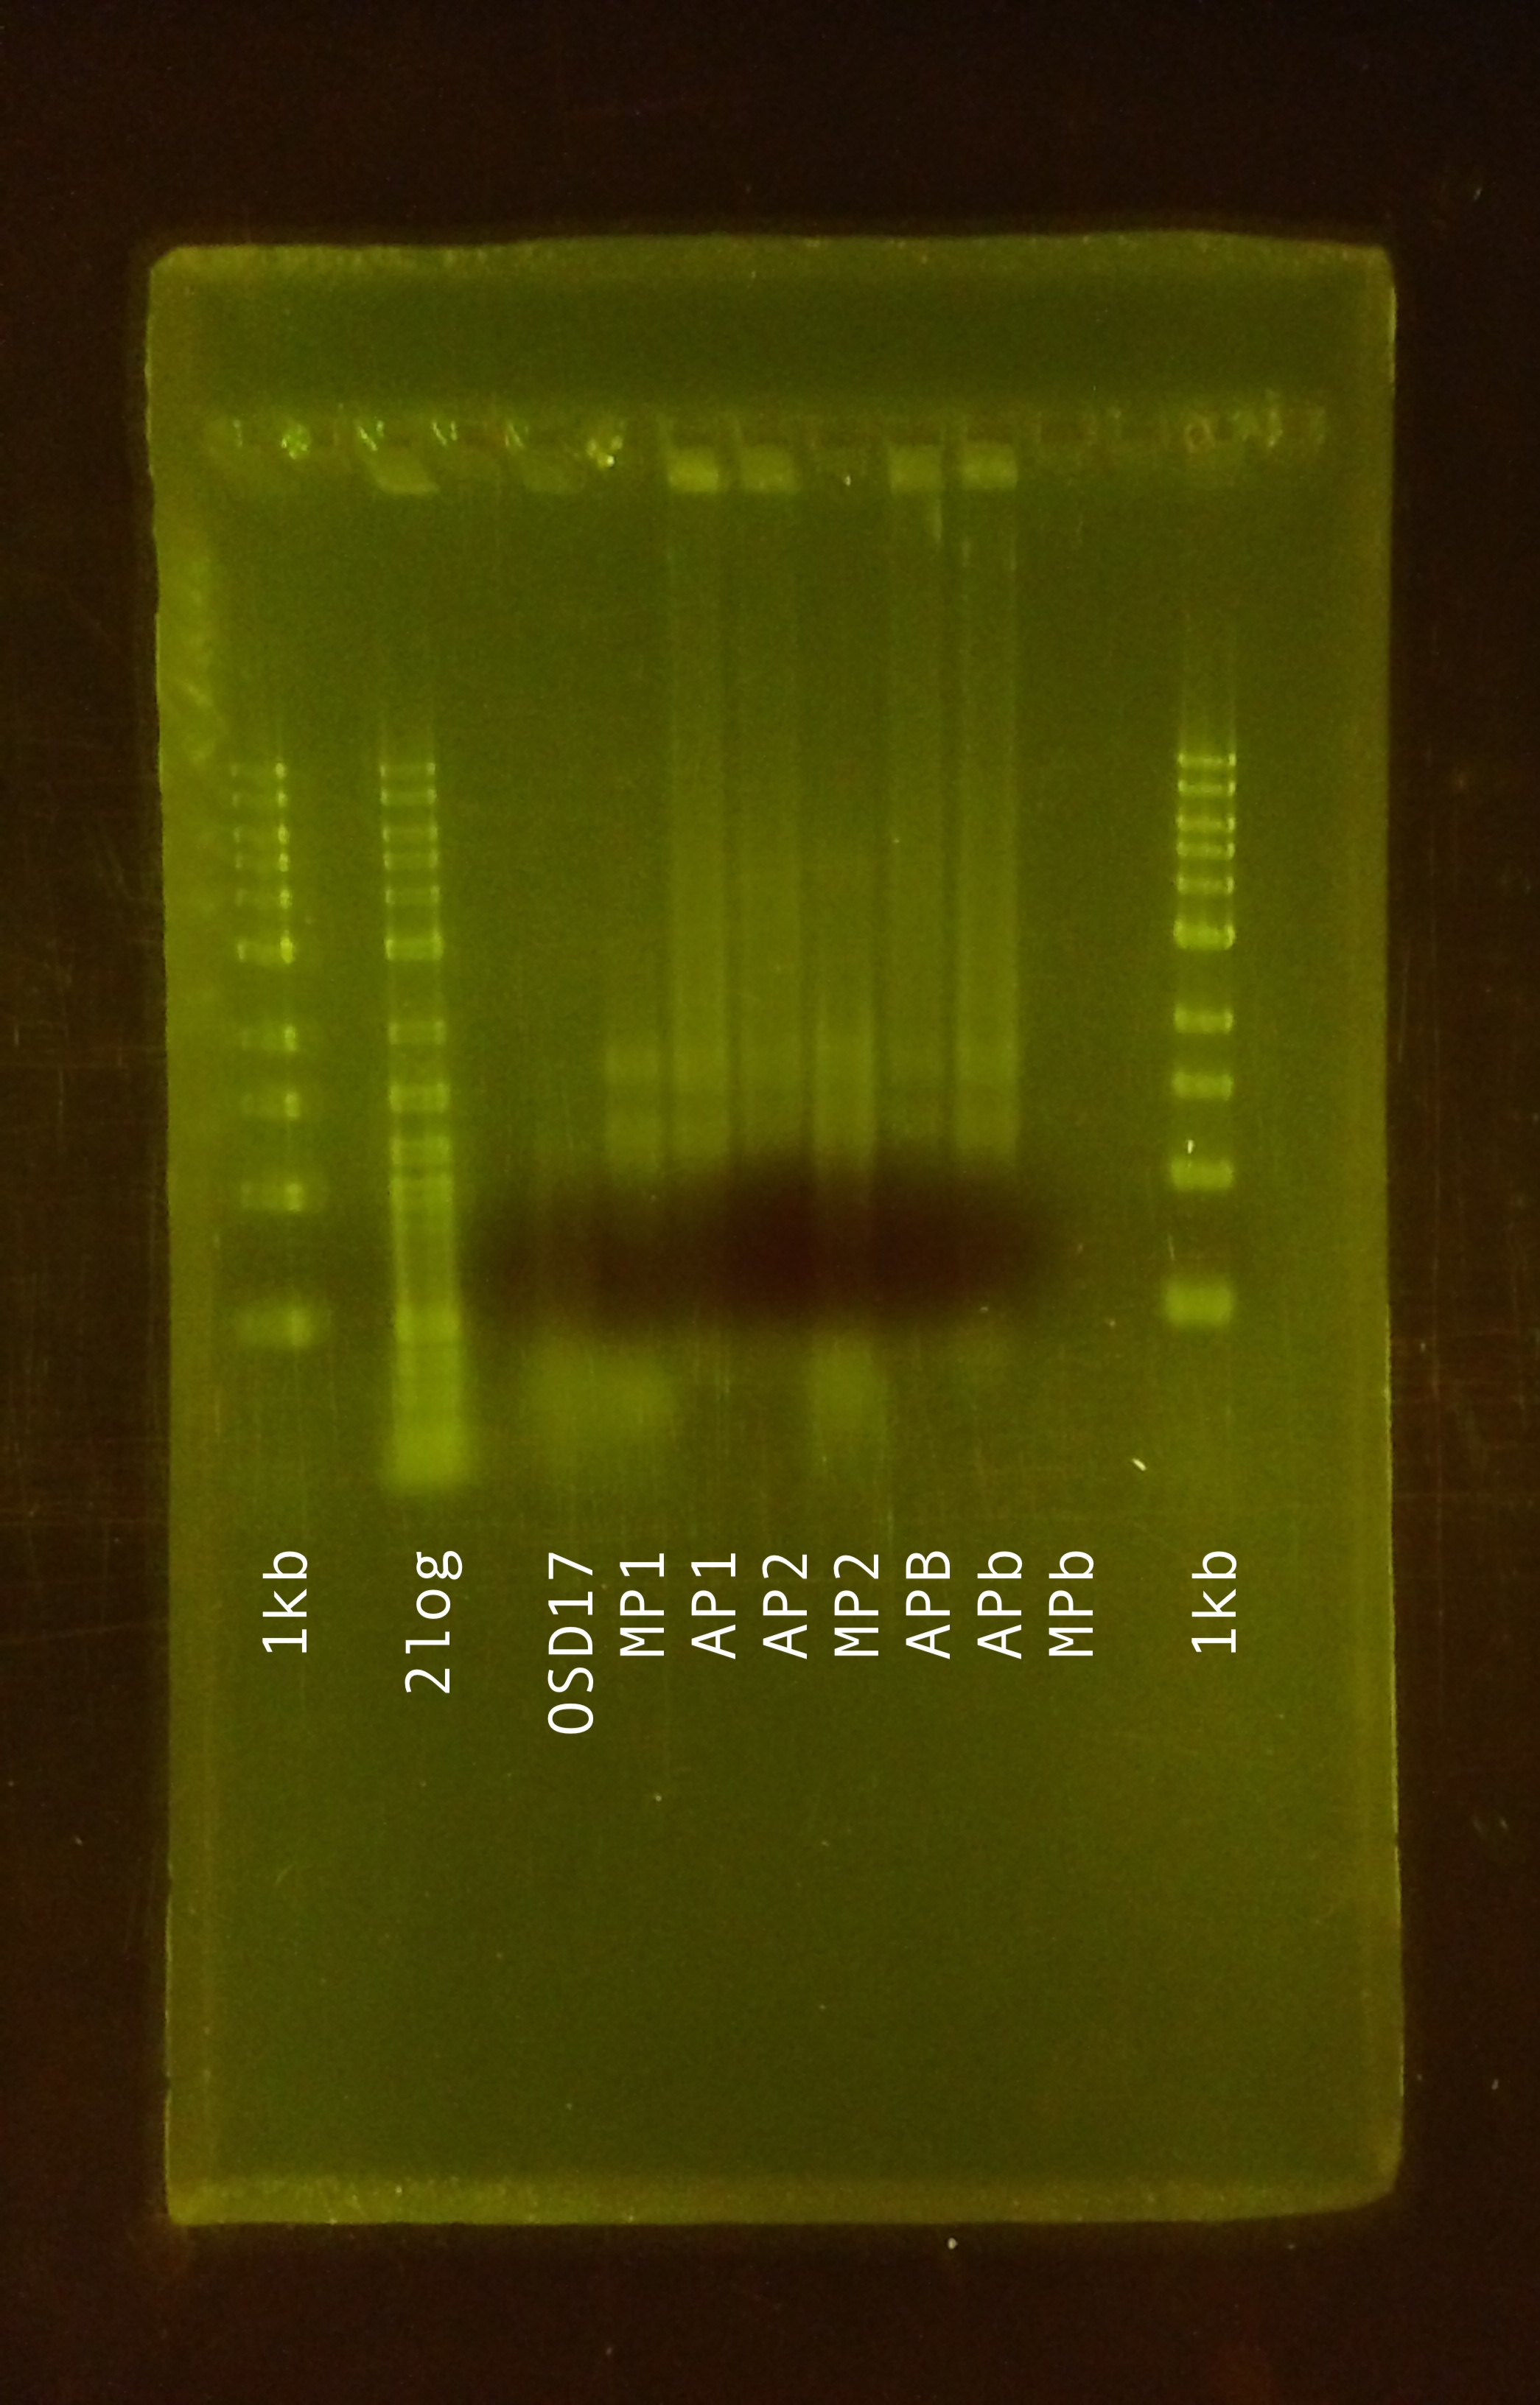
\includegraphics[width=0.4\textwidth]{graphics/pic/20180317_gel_sybr_gold_rna.jpg}
\end{figure}

Figure \ref{fig:20180317_gel_sybr_gold_rna} shows the gel with RNA samples after 60 min. migration and 30 min. staining in SYBR\cR Gold. It is possible to see the RNA samples except for sample labeled \texttt{MPb}: because the RNA concentration was very low, the volume I transfered to load 100 ng of RNA did not let me use a loading buffer, and when loading the sample in the gel, it did not fall at the bottom of the well and I lost the sample in the buffer ... 
As expected, sample \texttt{OSD} is the most degraded because it is the oldest sample. For all other samples, it is possible to see the bands corresponding to rRNAs (likely 16S and 23S). It seems that RNA extracted with MasterPure\texttrademark~ (\texttt{MP}) because it is possible to see smears at low molecular weight: small broken RNA fragment and nucleotides. 
Samples extracted with the AllPrep\cR mini kit seem to have better integrity with higher molecular fragments and no smears at the low molecular weight. 

\subsubsection{Conclusion}

I was able to assess the integrity of RNA samples by electrophoresis with SYBR\cR Gold stain. While it was not possible to determine which kit was the best when looking at DNA integrity, it is clear that AllPrep\cR kit allows to retrieve RNA with high integrity compared to the MasterPure\texttrademark~ kit. 

This is consistent with the quantity of nucleic acid extracted with these two kits, and it confirms that the RNA molecules very likely get damaged during the MasterPure\texttrademark~ protocol because it is longer and it involves a DNase treatment while AllPrep\cR is really quick and only relies on columns to separate DNA from RNA. 

These results reinforce my decision of using the AllPrep\cR kit.

